%% question-6.tex
%%

%% ==============================
\subsection{Diagramme d'un programme}
\label{sec:question6}
%% ==============================

Le diagramme présenté en figure \ref{fig:program}, représente une première version du langage \emph{Play}.
Un programme étant \guillemotleft simplement\guillemotright\ un ensemble de déclaration.

Une \emph{Declaration} hérite d'une classe virtuelle \emph{Named} qui permet de faire hériter, à l'ensemble des enfants de \emph{Declaration}, une propriété \emph{name}. 

\begin{figure}[h!]
	\centering
	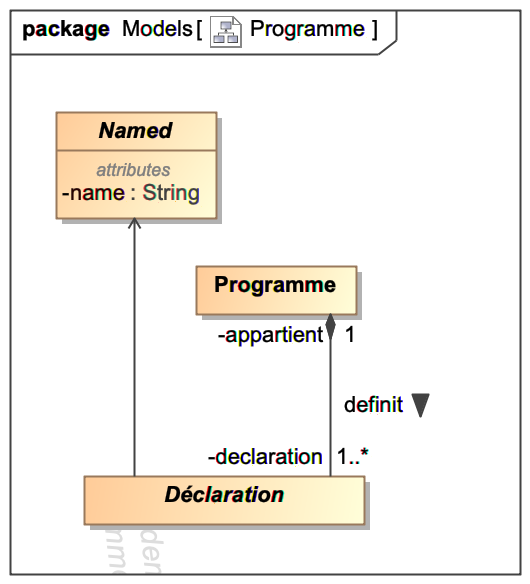
\includegraphics[width=300pt]{assets/class__Programme}
	\caption{Diagramme de classe d'un programme}
	\label{fig:program}
\end{figure}
